\section{Refactoring Implementation}
\subsection{JDisclosureToolBar class}





\subsubsection{initComponents}
This method now gives a clearer and more modular approach than before the Refactoring.
It initializes the layout of the toolbar and configures its components, including the disclosure button.

\textbf{Improvements:}
The refactoring makes it more readable and maintainable by breaking down the process into more clear steps steps,
thereby improving the overall structure of the code.

\begin{figure}[H]
    \centering
    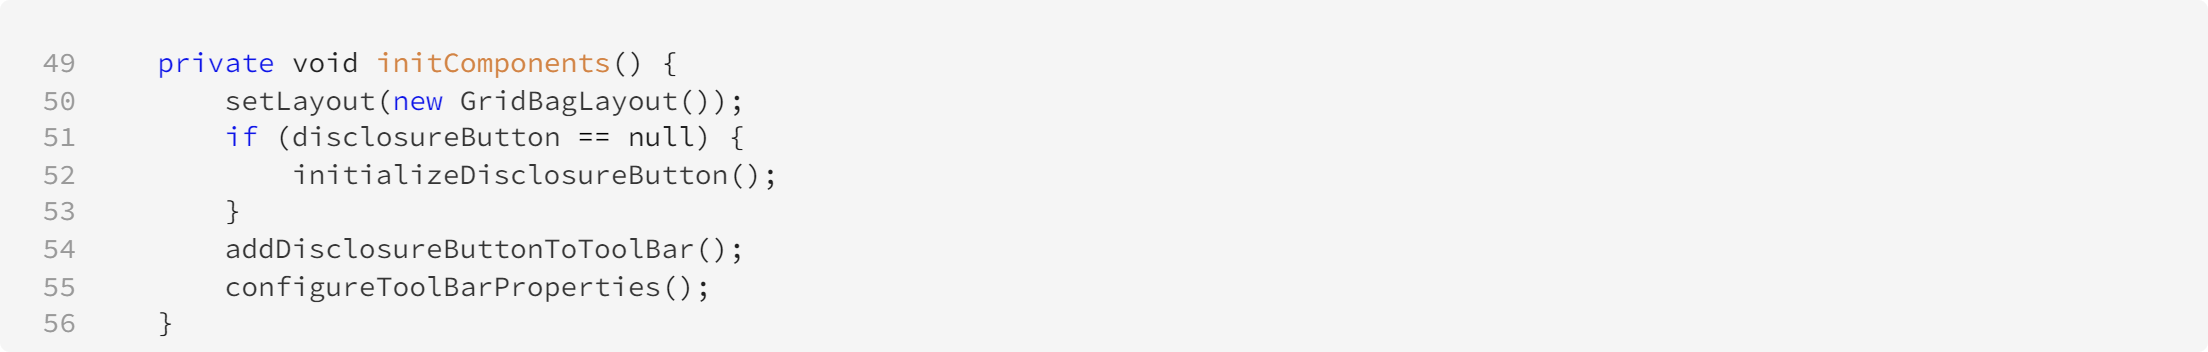
\includegraphics[width=\linewidth]{pic/F initComponents.png}
    \caption{Refactored initComponents Method}
    \label{fig:Refactored initComponents Method}
\end{figure}





\subsubsection{setDisclosureState}
This method manages the disclosure state of the toolbar, updating its state and rearranging components based on the new state.


\textbf{Improvements:}The refactoring of this method has streamlined it to be more clear and efficient than before.
By handling the state change and component rearrangement, it new enhance the toolbars adaptability state changes in the program.
with these Improvements its more readable and maintainable than before,
making it easier to understand and modify the toolbars behavior.

\begin{figure}[H]
    \centering
    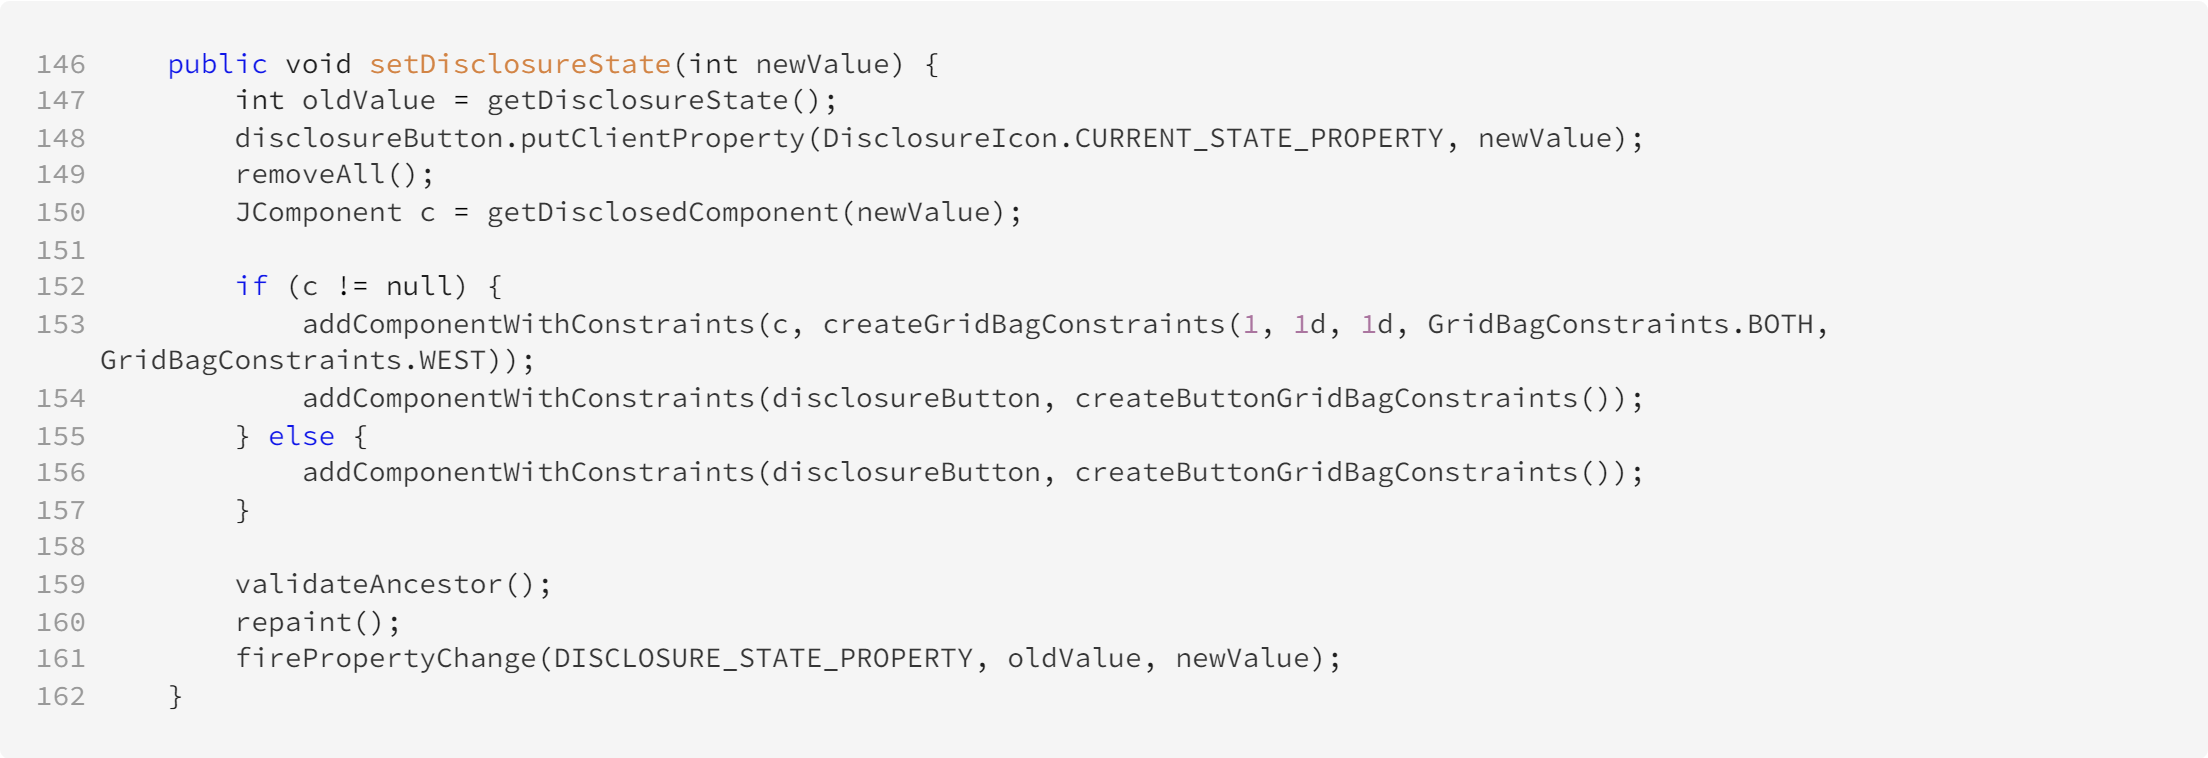
\includegraphics[width=\linewidth]{pic/F setDisclosureState.png}
    \caption{Refactored setDisclosureState Method}
    \label{fig:Refactored setDisclosureState Method}
\end{figure}






\subsubsection{initializeDisclosureButton}
The method is used to initializing the disclosure button, setting up its UI, and attaching an action listener for state changes,
to monitor when they happen.

\textbf{Improvements:} Separating the initialization of the disclosure button into its own method, to enhance the single responsibility principle,
making the code easier to understand and maintain by other developers.

\begin{figure}[H]
    \centering
    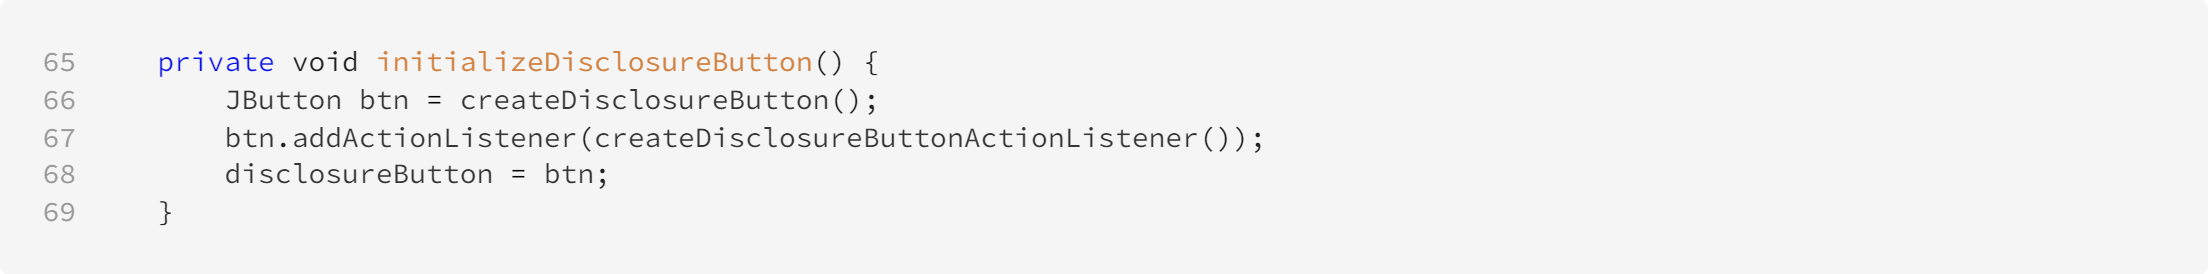
\includegraphics[width=\linewidth]{pic/F initializeDisclosureButton.png}
    \caption{Refactored initializeDisclosureButton Method}
    \label{fig:Refactored initializeDisclosureButton Method}
\end{figure}





\subsubsection{createDisclosureButton}
This method creates a JButton specifically configured as a disclosure button, setting its UI and properties.

\textbf{Improvements:} By encapsulating the creation of the disclosure button,
the code becomes more modular and reusable, promoting better coding practices.

\begin{figure}[H]
    \centering
    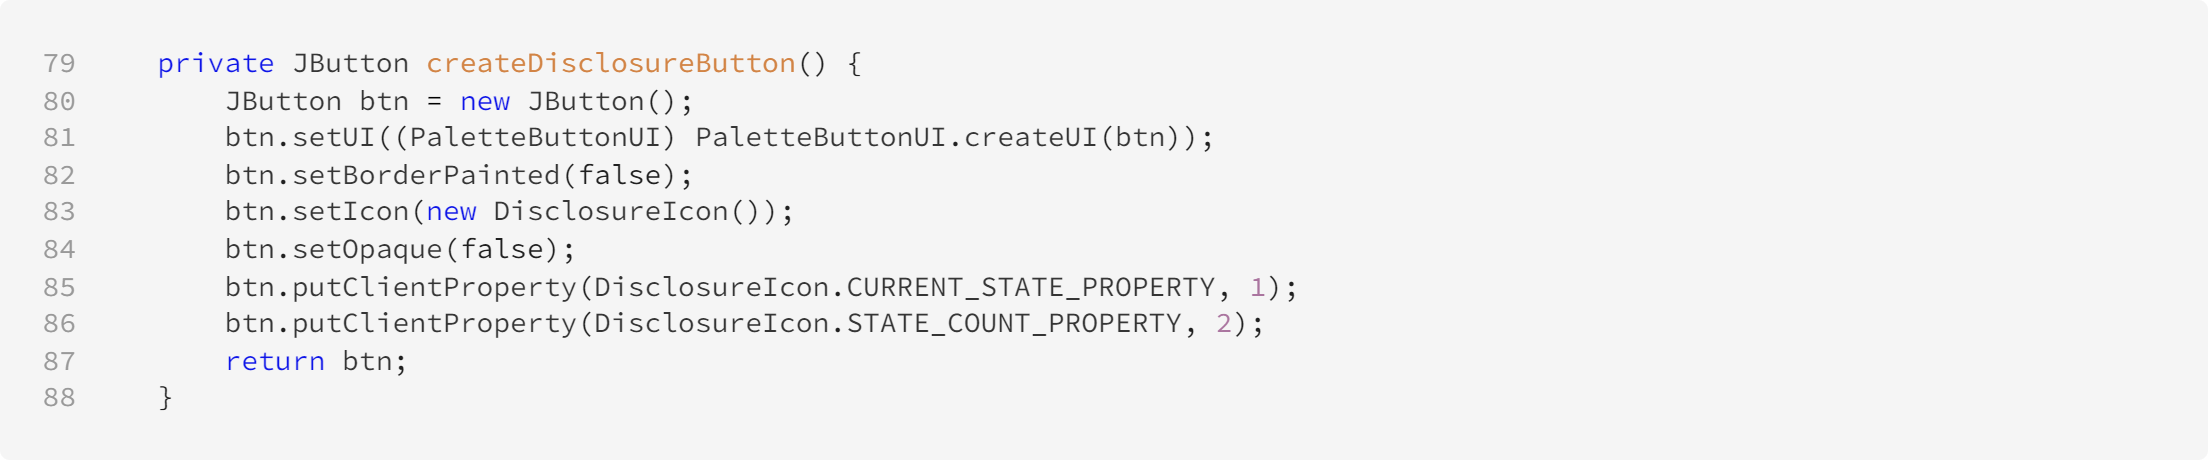
\includegraphics[width=\linewidth]{pic/F createDisclosureButton.png}
    \caption{Refactored createDisclosureButton Method}
    \label{fig:Refactored createDisclosureButton Method}
\end{figure}





\subsubsection{createDisclosureButtonActionListener}
This method creates an ActionListener for the disclosure button, handling the action when the changing the disclosure state of the toolbar happens.

\textbf{Improvements:}By isolating the action listener creation, it will improve the clarity of the event handling
and also simplify any modifications or extensions that might be needed in the future by other developers learning the system code.

\begin{figure}[H]
    \centering
    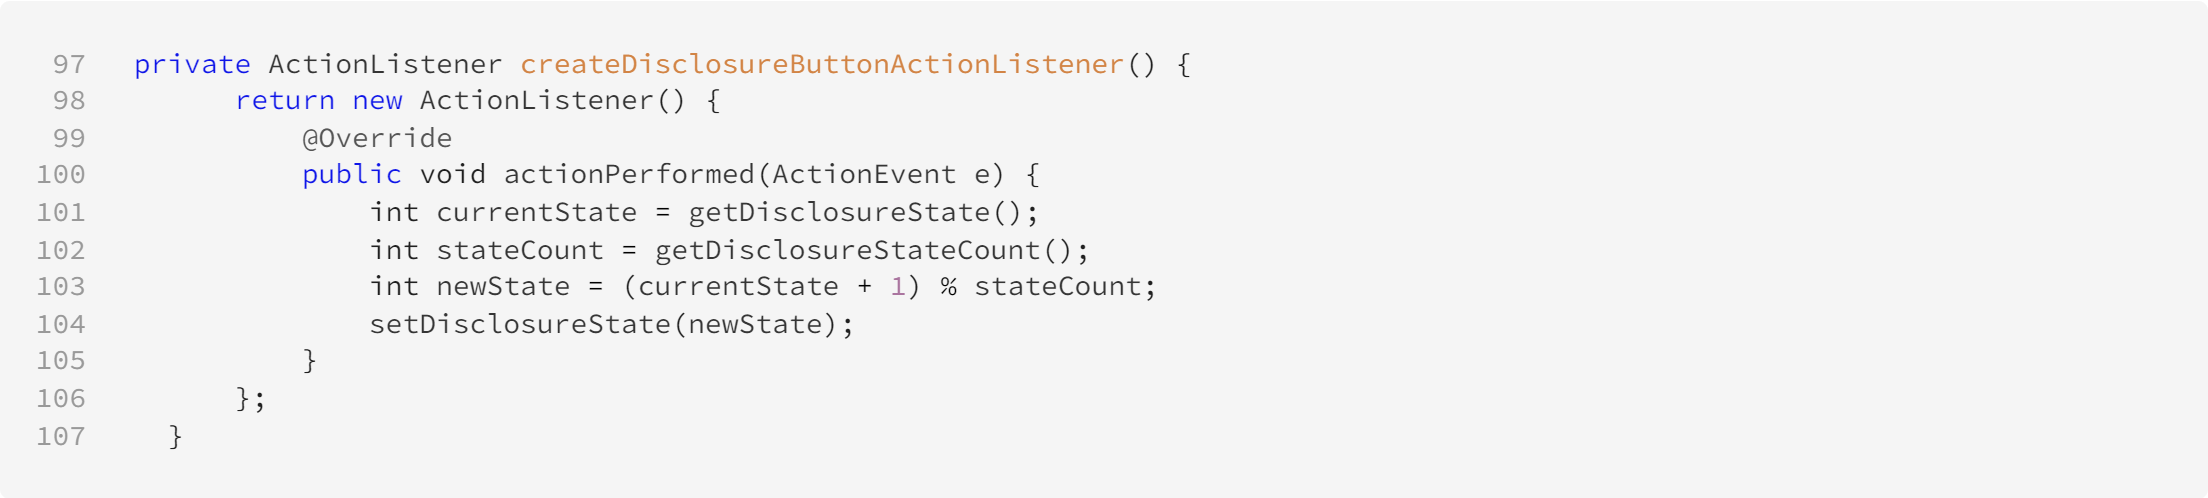
\includegraphics[width=\linewidth]{pic/F createDisclosureButtonActionListener.png}
    \caption{Refactored createDisclosureButtonActionListener Method}
    \label{fig:Refactored createDisclosureButtonActionListener Method}
\end{figure}



\subsubsection{addDisclosureButtonToToolBar}
This method adds the disclosure button to the toolbar with appthe right GridBagConstraints, it will handle the positioning within the toolbar it self.

\textbf{Improvements:} By isolating the process of adding the button to the toolbar,
the method will be more readable and make it easier to make any adjustments to the buttons positioning.

\begin{figure}[H]
    \centering
    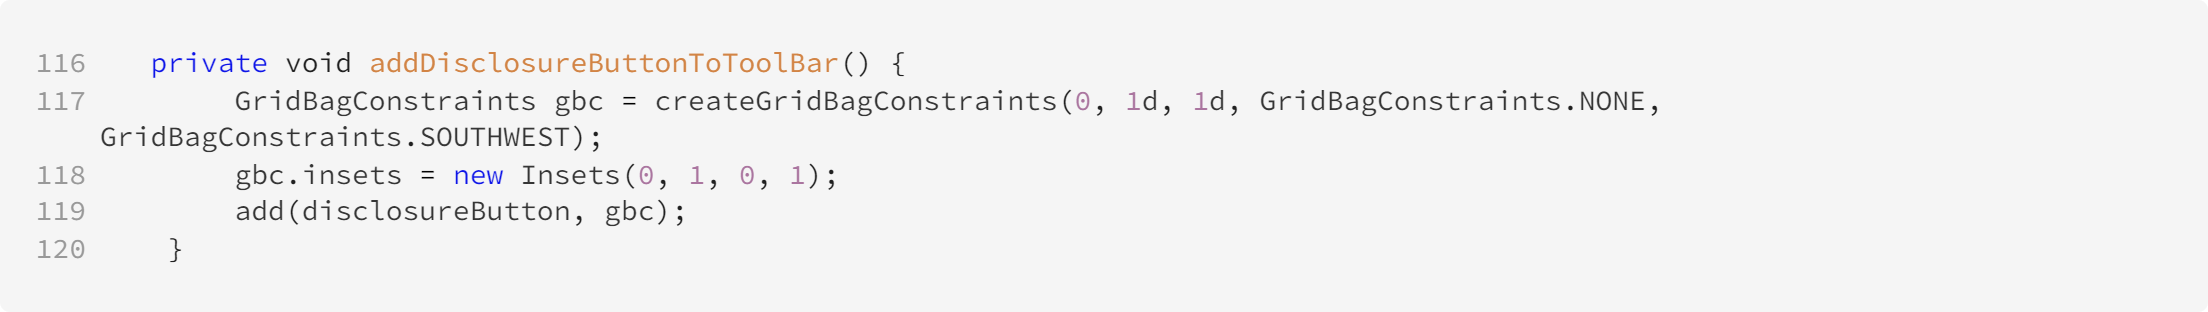
\includegraphics[width=\linewidth]{pic/F addDisclosureButtonToToolBar.png}
    \caption{Refactored addDisclosureButtonToToolBar Method}
    \label{fig:Refactored addDisclosureButtonToToolBar Method}
\end{figure}



\subsubsection{configureToolBarProperties}
this methods now sets up additional toolbar properties such as insets, icons and applying custom settings.

\textbf{Improvements:}This isolateds the method for additional set up aids in maintaining clean code and it will make
it easier to modify toolbar properties without affecting other functionalities of the toolbar palette.

\begin{figure}[H]
    \centering
    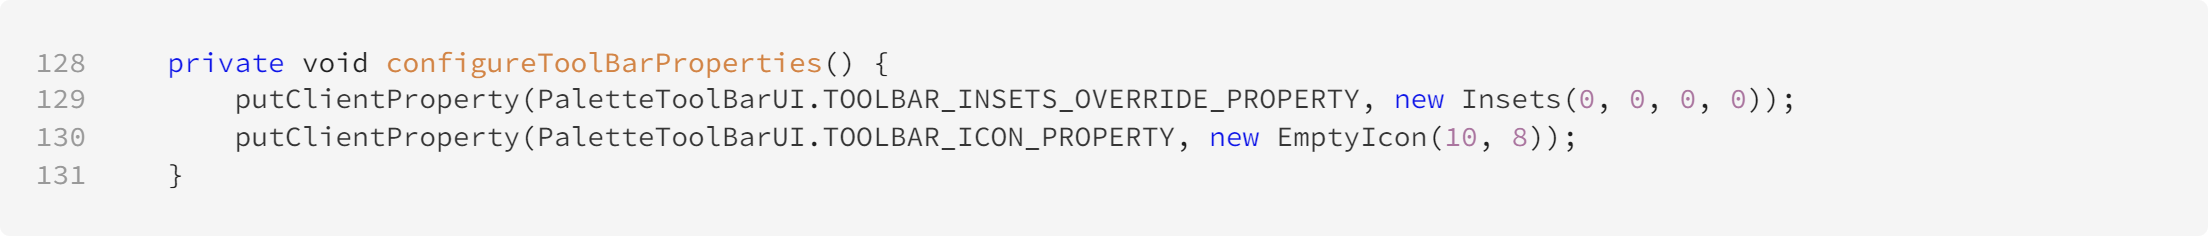
\includegraphics[width=\linewidth]{pic/F configureToolBarProperties.png}
    \caption{Refactored configureToolBarProperties Method}
    \label{fig:Refactored configureToolBarProperties Method}
\end{figure}





\subsubsection{validateAncestor}
Validates the ancestor container of the toolbar, making its the right layout and rendering shown the user.

\textbf{Improvements:} This method provides an method to validate the container hierarchy, which will
improving the dependability of the toolbars rendering process.

\begin{figure}[H]
    \centering
    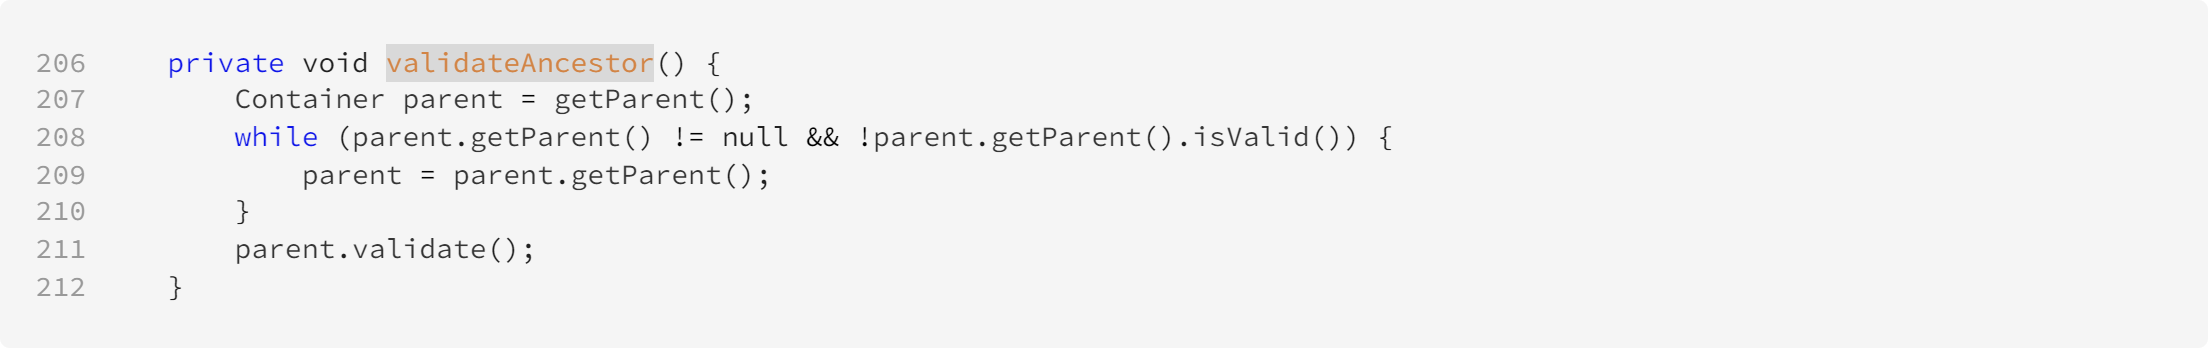
\includegraphics[width=\linewidth]{pic/F validateAncestor.png}
    \caption{Refactored validateAncestor Method}
    \label{fig:Refactored validateAncestor Method}
\end{figure}






\subsection{PaletteToolBarUI class - setFloating, dragTo and floatAt}





\subsubsection{setFloating}
This method is responsible for the floating state of the toolbar, it will choose whether it should be docked or floating based on the given parameters.

\textbf{Improvements:} The code is more readable and maintainable by breaking down the complex conditional logic into smaller methods with more clear responsibility,
than from before the refactoring.

\begin{figure}[H]
    \centering
    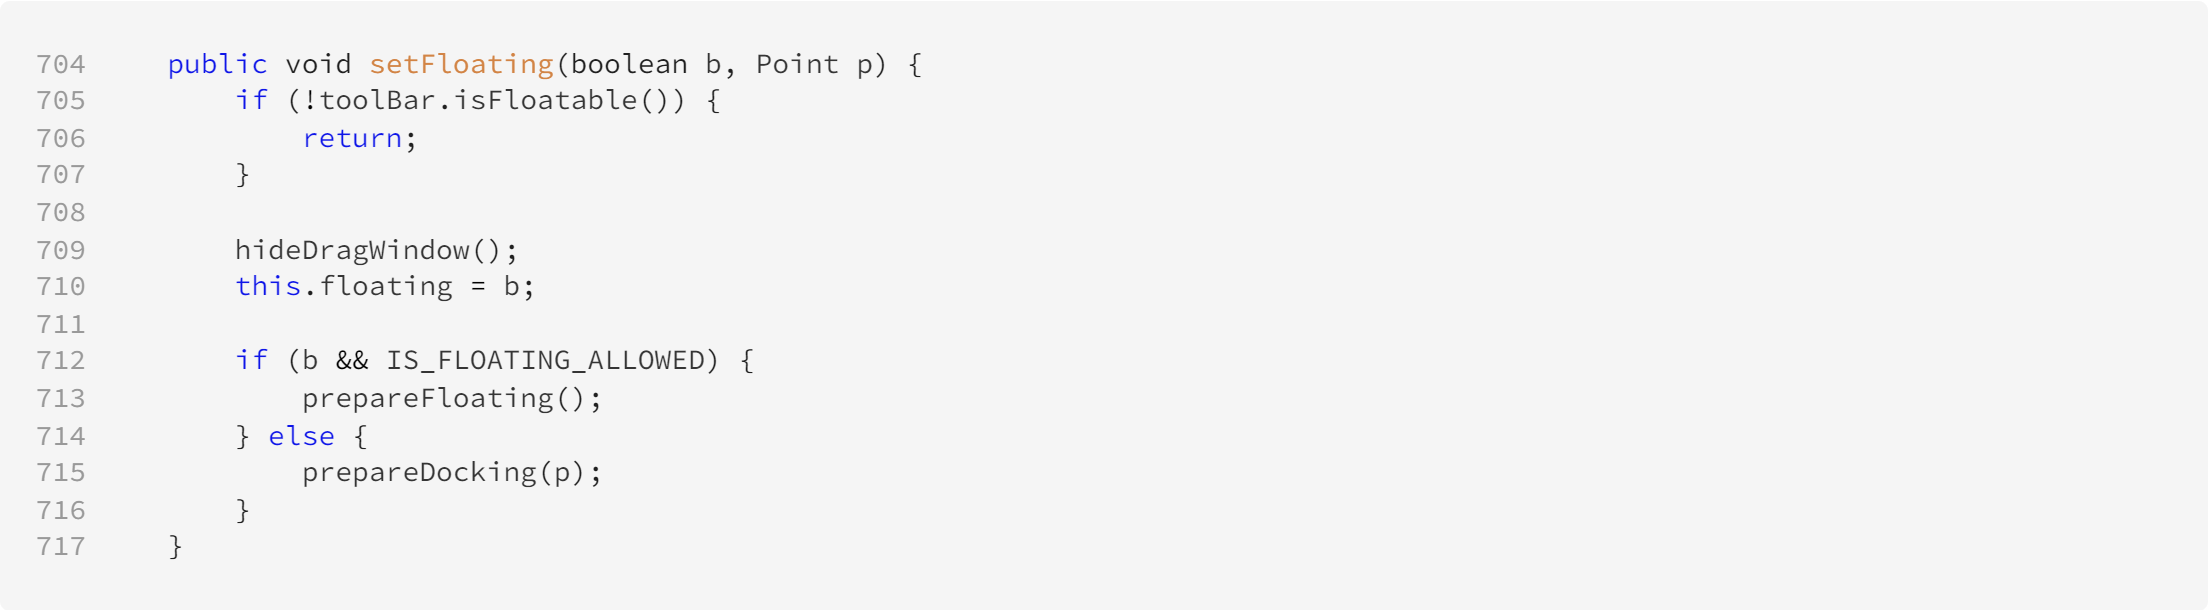
\includegraphics[width=\linewidth]{pic/F setFloating.png}
    \caption{Refactored setFloating Method}
    \label{fig:Refactored setFloating Method}
\end{figure}







\subsubsection{floatAt}
The method adjust the toolbars position, which is based on the current drag operation that is happening. It will be considering its floatability and docking potential doing so.

\textbf{Improvements:} Optimize the toolbars positioning during dragging of a toolbar, this is done by centralizing position calculations, leading to an more maintainable code
thats easier to read also.

\begin{figure}[H]
    \centering
    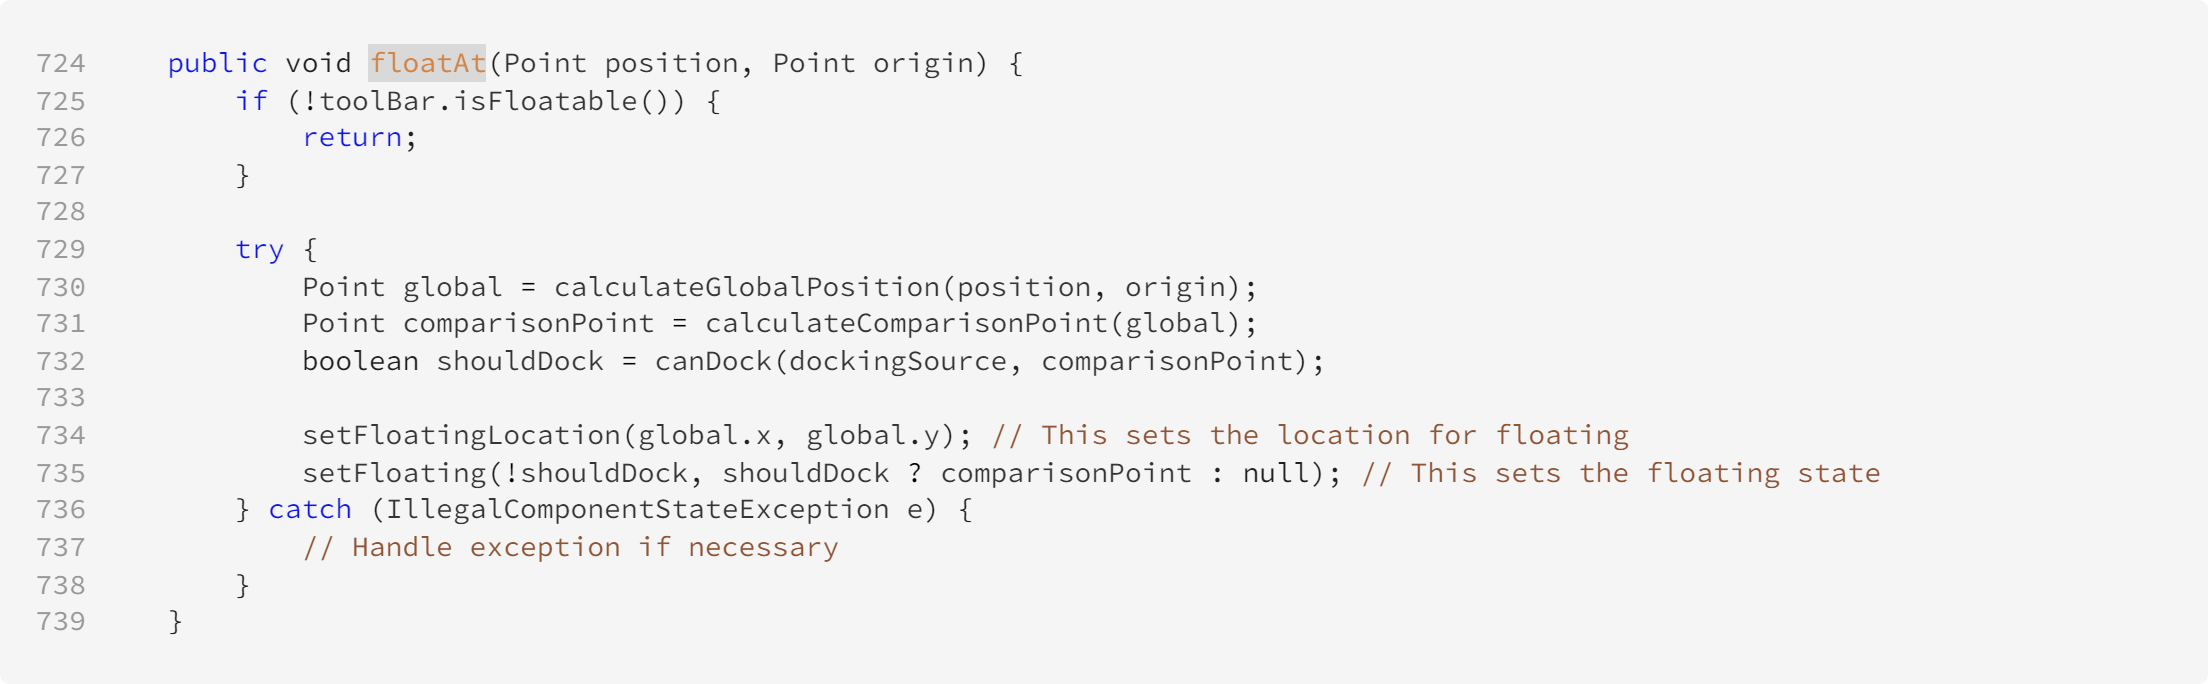
\includegraphics[width=\linewidth]{pic/F floatAt.png}
    \caption{Refactored floatAt Method}
    \label{fig:Refactored floatAt Method}
\end{figure}







\subsubsection{prepareFloating}
This method together wit the \textit{prepareDocking} method will separately handle the set up steps for floating and docking the toolbar.

\textbf{Improvements:} It now encapsulates the floating and docking actions, it also now have increased modularity and reducing complexity from than before the refactoring.

\begin{figure}[H]
    \centering
    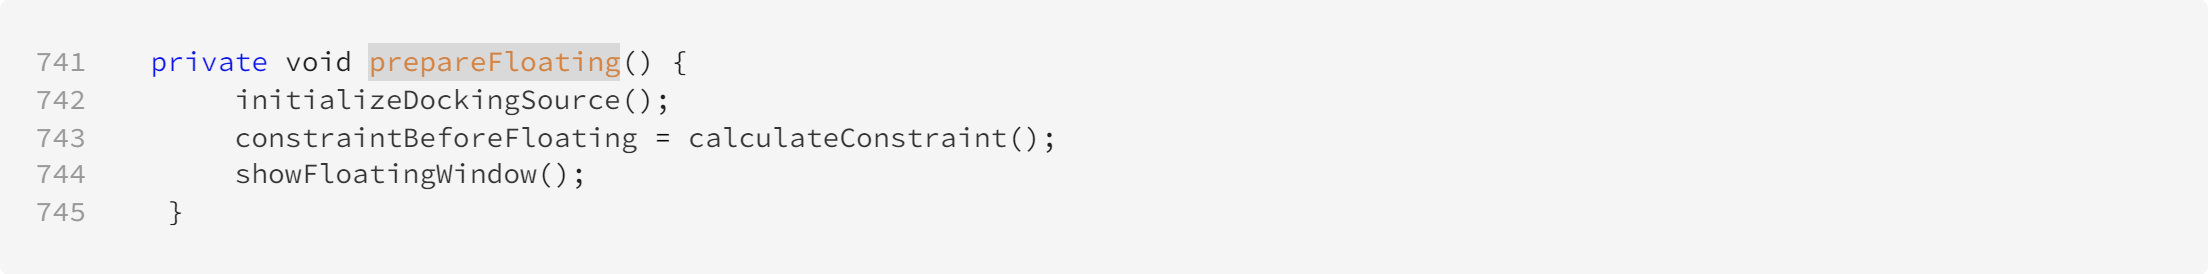
\includegraphics[width=\linewidth]{pic/F prepareFloating.png}
    \caption{Refactored prepareFloating Method}
    \label{fig:Refactored prepareFloating Method}
\end{figure}







\subsubsection{initializeDockingSource}
This method makes sure that the toolbars docking source is initialized before changing its floating state.

\textbf{Improvements:} By isolating the initialization of the docking source, it will be promoting code reuse and also simplifying the primary floating method at the same time.

\begin{figure}[H]
    \centering
    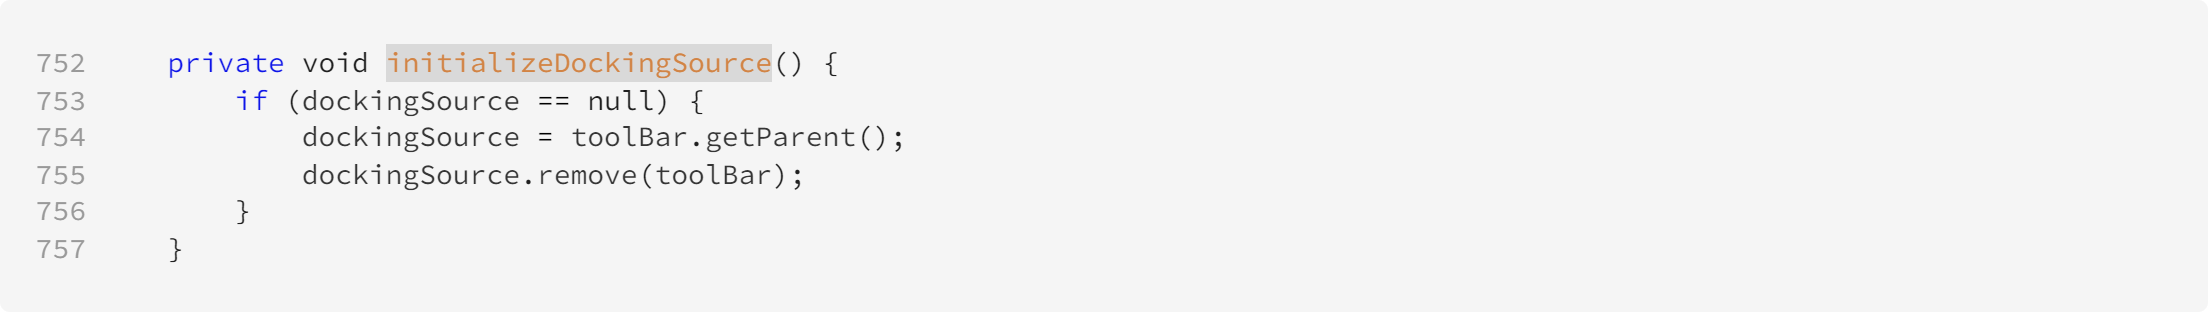
\includegraphics[width=\linewidth]{pic/F initializeDockingSource.png}
    \caption{Refactored initializeDockingSource Method}
    \label{fig:Refactored initializeDockingSource Method}
\end{figure}









\subsubsection{showFloatingWindow}
this method together with the metod \textit{updateFloatingWindowAppearance} will manage the visual presentation of the toolbar when it is in a floating state.

\textbf{Improvements:} By seperating the visual aspects of the old methods into new dedicated methods, will enhance the readability of UI changes and at the same time
simplifies the overall floating logic.

\begin{figure}[H]
    \centering
    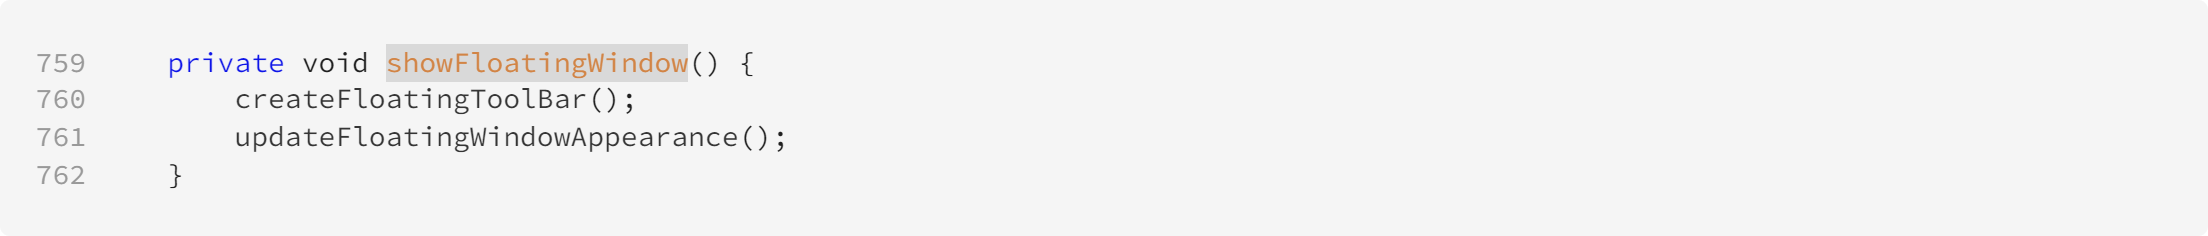
\includegraphics[width=\linewidth]{pic/F showFloatingWindow.png}
    \caption{Refactored showFloatingWindow Method}
    \label{fig:Refactored showFloatingWindow Method}
\end{figure}







\subsubsection{dragTo}
This methods is responsible for the toolbars dragging functionality, it will calculate and be setting the new position during a drag operation.

\textbf{Improvements:} By breaking down the dragging process into smaller steps, it will make the code and metod more readable and thereby the code easier to follow and maintain
by other developers in the future.

\begin{figure}[H]
    \centering
    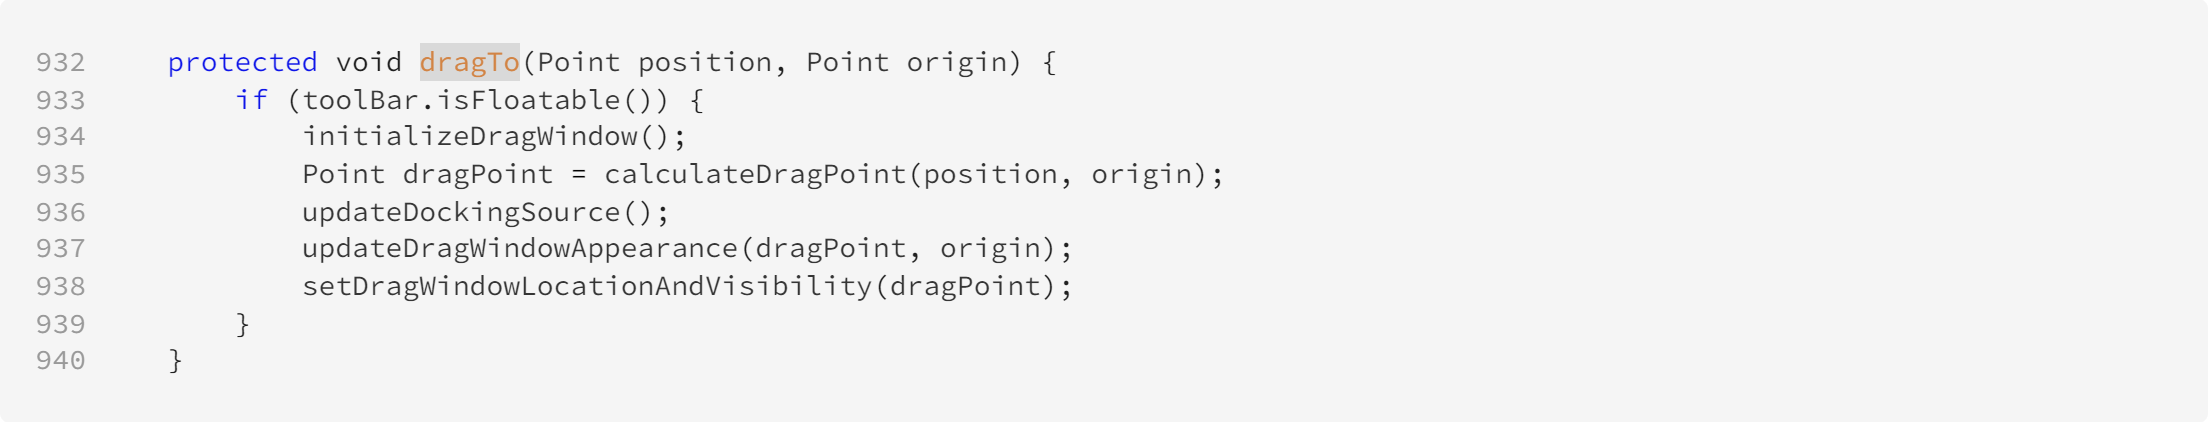
\includegraphics[width=\linewidth]{pic/F dragTo.png}
    \caption{Refactored dragTo Method}
    \label{fig:Refactored dragTo Method}
\end{figure}






\subsubsection{initializeDragWindow}
Together with the methods \textit{calculateDragPoint, getDragWindowOffset, updateDragWindowAppearance} and \textit{setDragWindowLocationAndVisibility} they will
together handle the initialization and appearance of the drag window, including its positioning and visibility.

\textbf{Improvements:} By make the code modular for the drag window functionality, it will enhance the structure and make it more maintainable,
by allowing each aspect to be modified independently of eachother.

\begin{figure}[H]
    \centering
    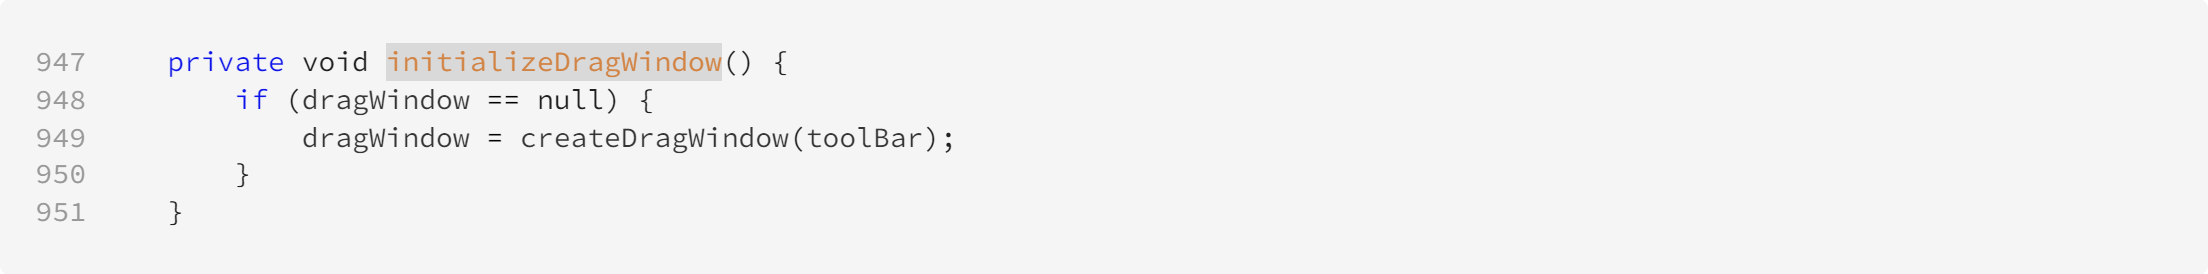
\includegraphics[width=\linewidth]{pic/F initializeDragWindow.png}
    \caption{Refactored initializeDragWindow Method}
    \label{fig:Refactored initializeDragWindow Method}
\end{figure}

\subsection{Impact of refactoring}
After having refactored the code for my feature \textit{Tool Palette}, there have been no breaking of the code or unexpected issues with other parts of the project.
Which is what was expected from the analysis of the code before the refactoring was performed. but there is still parts of the of code that could be refactored further,
but these parts of the code were not within the scope of the refactoring for my feature, but it could be something that could be done in the future by other developers.





